

\newpage

The term ``STEM" become a well-known acronym used by researchers, industry professionals, and practitioners across the globe (\cite{dugger2010evolution}, 2010). In 2001, the U.S. National Science Foundation (NSF) introduced this now popular acronym and expanded the scholarly interest in a collective study of the disciplinary areas of science, technology, engineering, and mathematics, or  STEM\footnote{\cite{hallinen2024} (2024) notes that the acronym `STEM' (science, technology, engineering, and mathematics) was the result of a NSF staff member rearranging the letters of the previously adopted term `SMET' (science, mathematics, engineering, and technology) or `SMT' (science, mathematics, technology).}. In the same year that the phrasing ``science, technology, engineering, and mathematics (STEM)" was introduced by NSF, the U.S. Congress also passed the \textit{No Child Left Behind Act of 2001} (NCLB). While various studies linked the passing of NCLB to racism (\cite{gay2007rhetoric}, 2007; \cite{lapayese2007understanding}, 2007; \cite{leonardo2007war}, 2007; \cite{taylor2006critical}, 2006; \cite{au2020testing}, 2020; \cite{wun2022anti}, 2022; \cite{taylor2006critical}, 2006), only recently have discourses about ``racism in STEM" increased in academic outlets. 

We explore how the co-location of historical influences helps to maintain dominant narratives and set the foundation for new eras of rhetoric in education research and policy (\cite{gay2007rhetoric}, 2007; \cite{standerfer2006before}, 2006).

\section{Meanings and notions}
\label{sec:meanings}

The introduction of the `STEM' acronym by NSF and the passing of NCLB by Congress in 2001 inform the primary basis of this study. We use these historical cases to map the research on the conceptual implications of concerns related to a largely assessment and testing focused era. NCLB, like previous Acts of U.S. Congress, would prove to be a major driver of education research (\cite{cawelti2006side}, 2006; \cite{groen2012nclb}, 2012; \cite{sunderman2005nclb}, 2005) and it would inform forthcoming Acts and national policies (see, e.g., the Every Student Succeeds Act, \cite{mathis2016lessons}, 2016). While multiple scholars have discussed the intersection of NCLB policies and racism, only recently due we see a rise in research on racism in STEM. In this article, we consider the historical development of research on racism in STEM by examining a corpus of texts published during the period of this intersection that prompted hyperactivity in the educational sciences.

We find that


\newpage

The identification of citation patterns (Who cites whom?) and citation communities (Who is relevant to whom?) is an important area of inquiry, especially for more recent topics of study and new disciplinary areas of study. In traditional bibliometric analysis and visualization -- the analysis of scientific publications and data -- the inclusion of citation patterns is standard but alone, they are marked by limitations (\cite{gingras2008effects}, 2008). 

Despite extensive funding, politics, and ongoing divisions resulting from these intersecting moments, visible structures of racialization and racism continue to impact educational opportunity and can be observed uniquely in the contexts of STEM. 

discourses across academic disciplines and areas of study requires an increasingly complex, multidisciplinary, and multifaceted approach. As software developers and engineers continue to provide new tools to improve efficient access to information stored in databases, there is an increase in concerns about the way that certain information is codified and stored. Moreover, as researchers develop insights based on these stored data, it is important to consider not only who uses certain systems, but the variations that will exist across new computational tools. 


% Please add the following required packages to your document preamble:
% \usepackage{multirow}
% \usepackage{lscape}
\begin{landscape}
\renewcommand{\arraystretch}{1.05}
\begin{table}[]
\centering
\caption{Inclusion and exclusion criteria for study data}
\label{tab:criteria}
\begin{tabular}{llll}
\hline
 &
  \textbf{Code} &
  \textbf{Criteria} &
  \textbf{Note(s)} \\ \hline
\multirow{5}{*}{Inclusion criteria (IC)} &
  IC 1 &
  \begin{tabular}[c]{@{}l@{}}Article contains both of the\\ core terms in either the title,\\ abstract, or keywords\end{tabular} &
  \begin{tabular}[c]{@{}l@{}}We conducted a search with the two core terms for the\\ study using the logical AND string operator\end{tabular} \\ \cline{2-4} 
 &
  IC 2 &
  \begin{tabular}[c]{@{}l@{}} Article was published after \\ 2001 and before 2024\end{tabular} &
  \begin{tabular}[c]{@{}l@{}}The earliest search date in WoS was 1992; the collections \\ selected for this study had an earliest date of 2002\end{tabular} \\ \cline{2-4} 
 &
  IC 3 &
  Article is written in English &
  Only articles originally written in English were considered \\ \cline{2-4} 
 &
  IC 4 &
  \begin{tabular}[c]{@{}l@{}}Article is a research article \\ in a peer-reviewed journal\end{tabular} &
  \begin{tabular}[c]{@{}l@{}}Only research articles published in peer-reviewed journals \\ and indexed by WoS or included in the ERIC databases \\ were included; e.g., no editorials were included\end{tabular} \\ \cline{2-4} 
 &
  IC 5 &
  \begin{tabular}[c]{@{}l@{}}Article problem, purpose, or\\ core question(s) relate(s) to\\ the keywords for the study\end{tabular} &
  \begin{tabular}[c]{@{}l@{}}While an indexed source may use core words for the study, \\ only articles that focused on both words were included\end{tabular} \\ \hline
\multirow{2}{*}{Exclusion criteria (EC)} &
  EC 1 &
  \begin{tabular}[c]{@{}l@{}}Articles not containing key \\ bibliometric source content\end{tabular} &
  \begin{tabular}[c]{@{}l@{}}Articles that had missing information on any key \\ study variables were excluded\end{tabular} \\ \cline{2-4} 
 &
  EC 2 &
  \begin{tabular}[c]{@{}l@{}}Articles that were non-standard\\ or non-research journal content\end{tabular} &
  \begin{tabular}[c]{@{}l@{}}Articles containing ancillary content (e.g., editorials \\ for a special issue; lectures or speeches) were excluded \end{tabular} \\ \hline
\end{tabular}
\end{table}
\end{landscape}

\section{Data and Methods}
\label{sec:data}



Our use of the term 'notion' also comes with attention to the ways that context contributes to scholarly literature. In this way, we examine the variations across geographical groupings and country ascriptions. We focus primarily, however, on the co-occurence of terms to make sense of the varied contexts in which the notions identified in the study inform. We also examine the use of historical scholarship in contemporary researchers' discourses.



We conduct an analysis  

\section{Conclusion}
\label{sec:conclusion}

In this article, we conclude that education researchers and those publishing in education journals are primary supporters of an interdisciplinary exchange of ideas, concepts, and keywords in the study of racism in STEM.

\newpage

We examine various notions of the term $racism$ in the context of scholarly discourses on science, technology, engineering, and mathematics (STEM). Sample data was extracted from a series of computational software systems using logic-based commands. By doing so, we examine the common practice of information retrieval (\cite{chowdhury2010intro}, 2010; \cite{kobayashi2000info}, 2000) and from a quantitative historical lens. We begin by outlining how researchers' use and contextualization of a key term, and a set of related keywords, can vary by discipline and terminal, defined by the availability of data, key historical points, or periods of interest. We explore how results vary by the varied computational tools utilized by researchers and, in effect, are further impacted by a set of disparate social, historical, and technological forces.

In summary, there is a pressing need to advance our understanding of the typologies of racism and their functions across various contexts, with a particular focus on STEM fields. By critically examining hidden conditions and adopting a nuanced approach, we can contribute to the broader discourse on combating racism and fostering inclusivity within academic and professional spheres.




Many traditional synthesis studies, meta-analyses, and bibliometric analyses focus on associations and major themes. In this study, we attended to the nuances that are produced by common practices as technologies change and new computational tools emerge. When doing so, a host of new questions emerged. These questions include some of the more traditional approaches to the analysis of journal articles, and sought to integrate critiques of various social components. In doing so, a key question was centered: \textit{What are the varying notions and typologies of racism and related keywords used by scholars in studies of science, technology, engineering, and mathematics}?

\section{Study results}

\subsection{Discipline and field of study associations}

%\end{landscape}
% 106 other categories
% Other & 92 & 18.42 \\



We found that the majority of articles published at the intersection of racism and STEM were authored by scholars in the United States. A total of 352 articles, comprising 74.26\% of the publications, originated from the United States. Ten percent (10\%) were published in England, amounting to a total of 35 articles. In Canada, there were 31 articles published, accounting for 6.54\% of the total. Australia had 19 articles published, making up 4\% of the total. These top four countries serve as one historical component of our study, allowing us to explore various historical markers that conceptually relate to the study of racism in STEM.

\begin{figure}[h]
\caption{Three-field plot of country, author, and keywords (N = 251)}
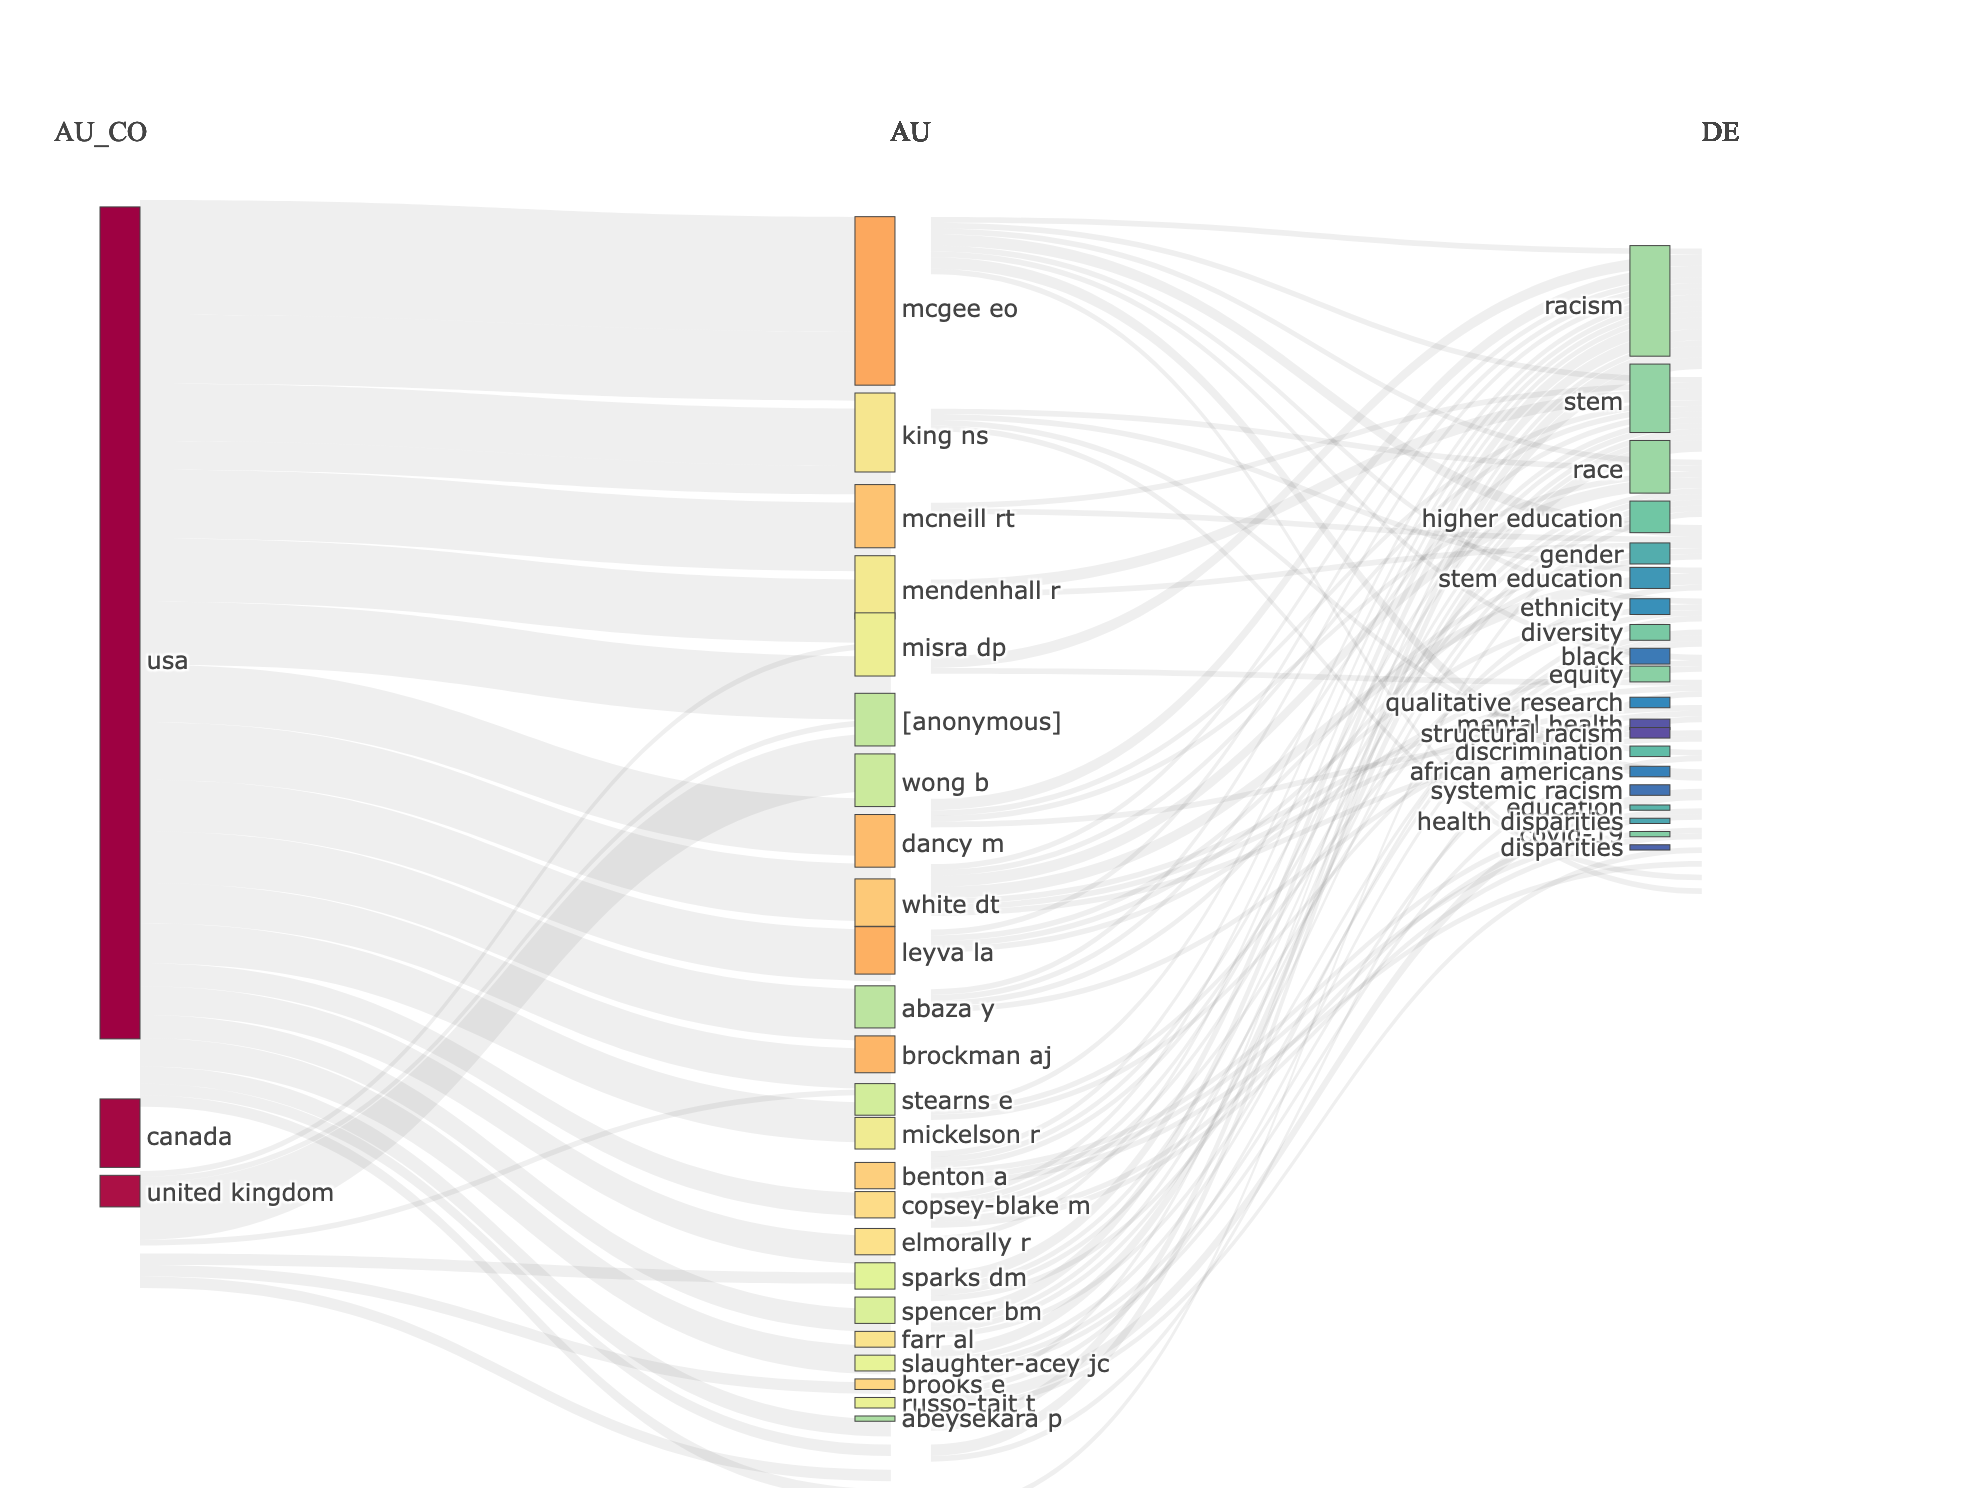
\includegraphics[width=16cm]{three-field-author-country.png}
\end{figure}


\begin{figure}[h]
\caption{Three-field plot of keywords, keywords-plus, and country (N = 251)}
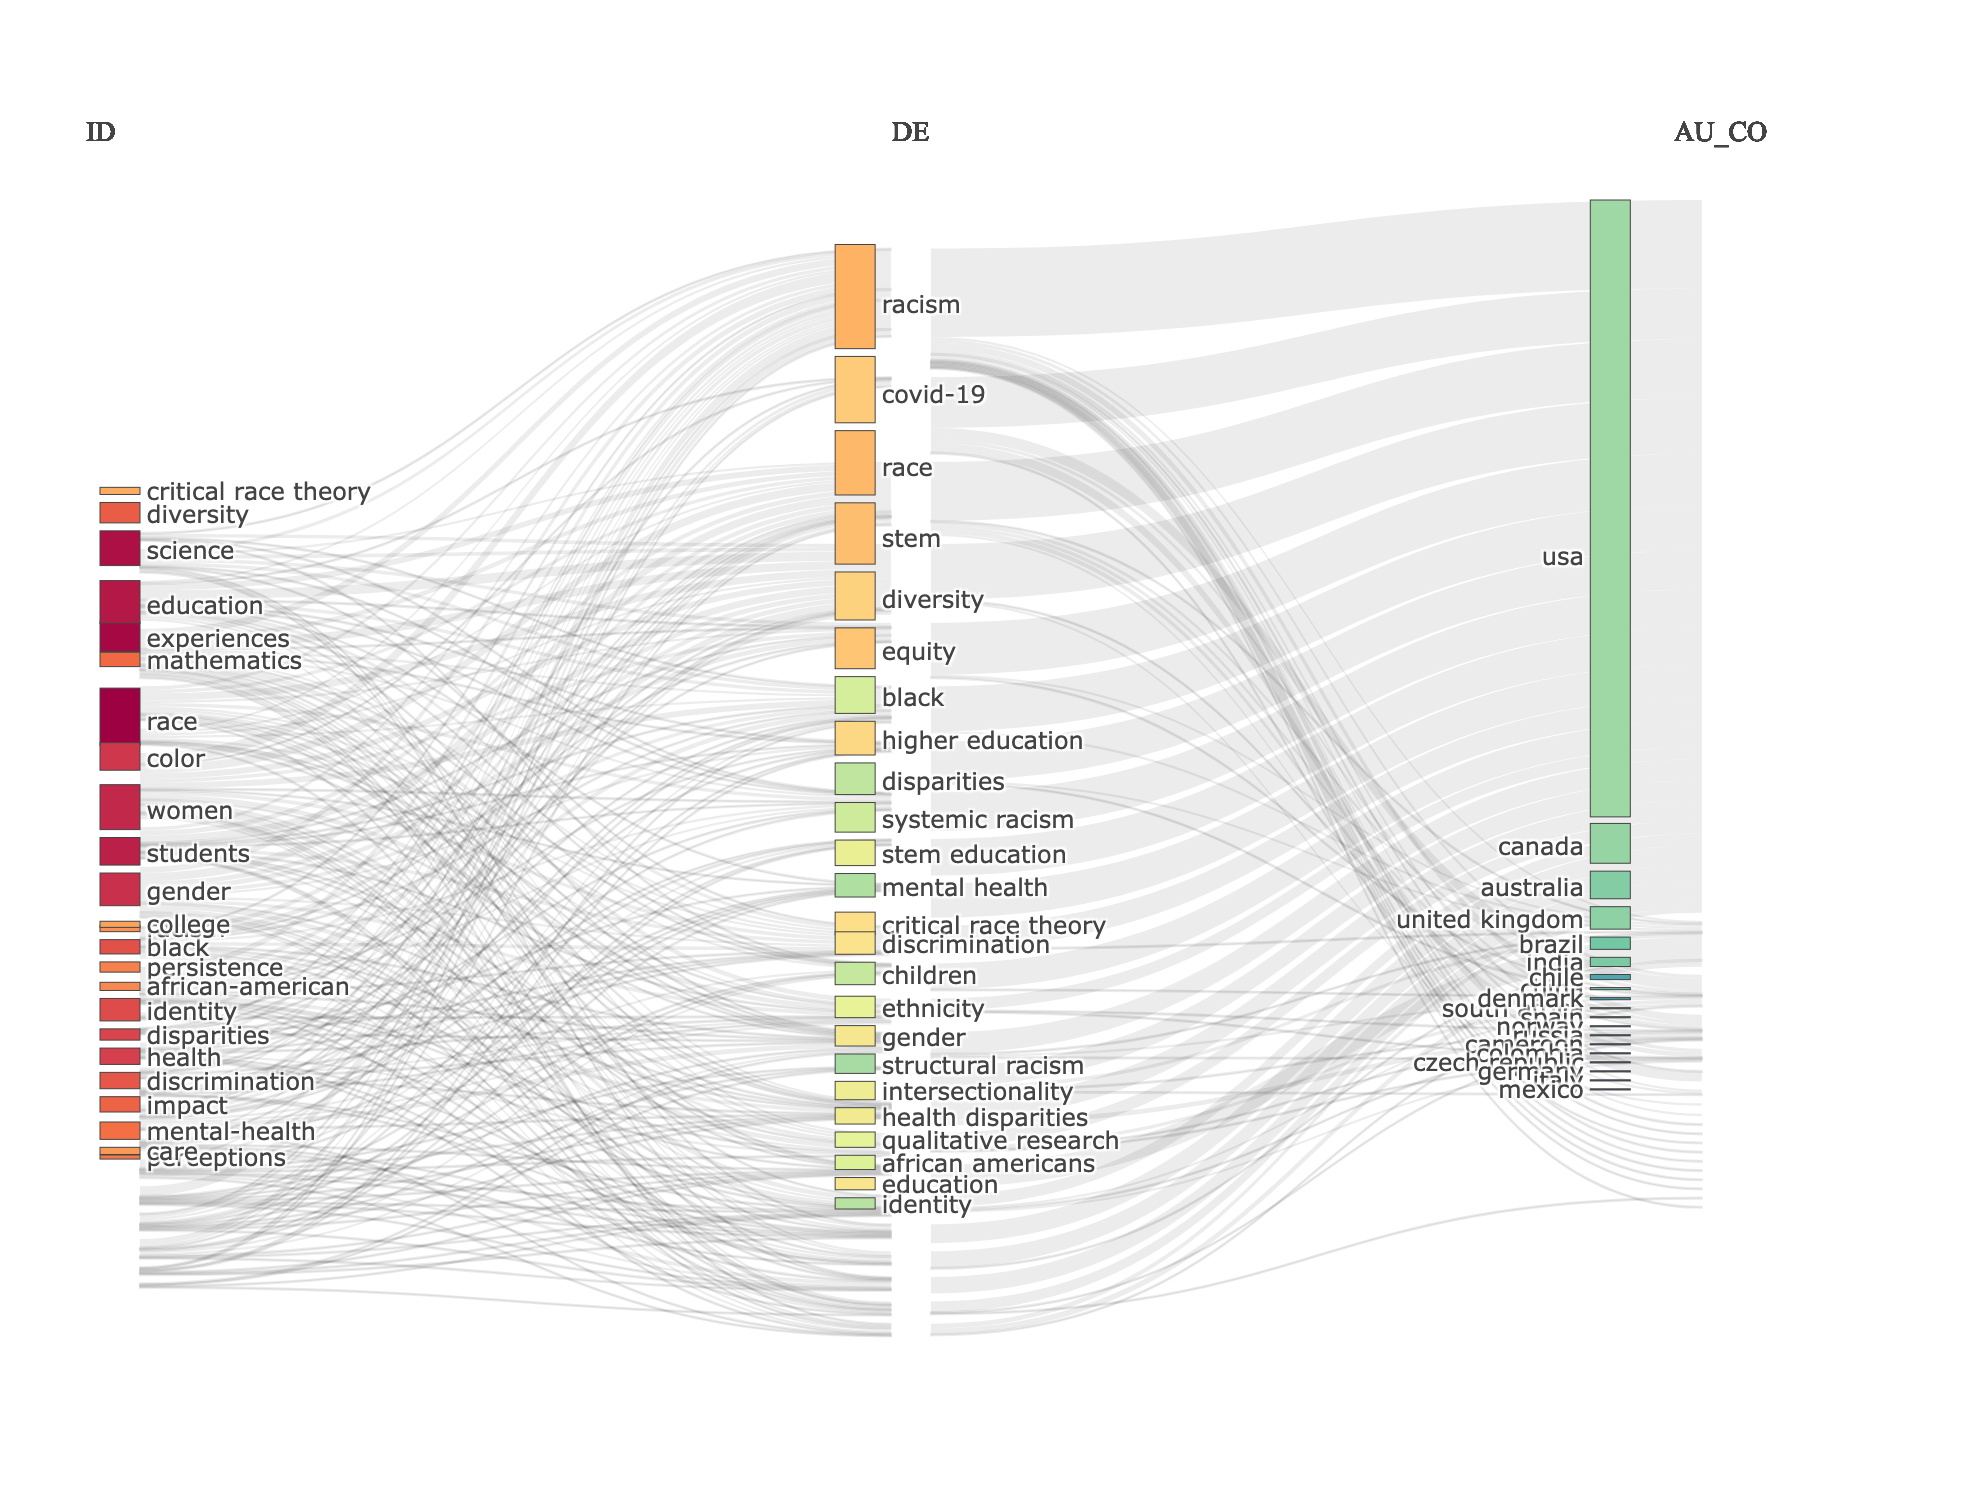
\includegraphics[width=16cm]{three-field-keywords-keywords-plus.png}
\end{figure}

In the United States, the Civil Rights Act of 1964 includes Title VI, which prohibits exclusion based on race, color, or national origin in relation to federal financial assistance. In England, the Race Relations Act of 1965 was the first legislation in the United Kingdom to explicitly address racial discrimination. This act outlawed various forms of discrimination based on color, race, ethnic or national origins in public places in Great Britain. It is important to note the distinction between the Race Relations Act and the Civil Rights Act in relation to public spaces and places receiving federal financial assistance.

In Canada, the Human Rights Act of 1985, despite its title, focuses on equal opportunity for individuals. It prohibits discrimination on various grounds, including race, national or ethnic origin, color, religion, age, sex, sexual orientation, gender identity, marital status, family status, genetic characteristics, disability, and conviction for any offense for which a pardon has been granted. Although the Canadian Human Rights Act does not explicitly use the term ``racism" in its title, it addresses discrimination comprehensively.

Finally, in Australia, the Racial Discrimination Act of 1975, administered by the Australian Human Rights Commission, makes it unlawful to discriminate against a person based on their race, color, descent, national origin, or ethnic origin, as well as their marital status. When considering these four countries, we observe various historical markers that have potentially influenced the development of federal-level laws, shaping researchers' perspectives on race schism. Notably, the United States holds significance in understanding the broader social context of studying racism.

We take note that a majority of these federal laws were passed in the 1960s, 1970s, and 1980s. As a result, we were interested in understanding the limitations of the WoS database and considered other sources of data that might inform some of the literature related to these markers and related keywords or terms. We use the ERIC database given its focus on federal matters in the United States, as one example of a needed intersection of modern computational tools and historical considerations. We present the results of this exploration in the next section.

%%% DATA - RPYS
% \begin{figure}[h]
% \caption{Reference spectroscopy from earliest citation in sample}
% \includegraphics[width=16cm]{reference_spectroscopy_1894_2023.png}
% \end{figure}



\begin{figure}[h]
\caption{Keyword co-occurence network (N = 251)}
\includegraphics[width=16cm]{co-occurence-network.png}
\end{figure}

\begin{landscape}
\begin{centering}
\begin{figure}[h]
\caption{Keyword thematic network (N = 251)}
\includegraphics[width=28cm]{thematic-mapping-network.png}
\end{figure}
\end{centering}
\end{landscape}


\begin{landscape}
\begin{centering}
\begin{figure}[h]
\caption{Factorial Analysis (N = 251)}
\includegraphics[width=25cm]{factorial_analysis_related_terms.png}
\end{figure}
\end{centering}
\end{landscape}


%%%%%%%%%%%%%%%%%%%%%%%
%%%%%%%%%%%%%%%%%%%%%%%

We then return to the full study sample to further identified notable associations in the databases.

%%%% table: 
\renewcommand{\arraystretch}{1.25}
\begin{table}[h]
\caption{Differences in keyword returns by database and search pattern}
\centering
\begin{tabular}{llrrrr}
\toprule
           &             & \multicolumn{4}{c}{Database}                    \\
           \cmidrule{3-6}
           & {Pattern}     & {ERIC} & {Google Scholar} & {Scopus} & {Web of Science} \\
           \midrule
Scenario 1 & racism      &      &                &  52,549      &  38,904              \\
Scenario 2 & race        &      &                &    376,723    &    301,024            \\
Scenario 3 & rac*        &      &                &        &    844,945            \\
Scenario 4 & racism stem &      &                &        &   499             \\
Scenario 5 & race stem   &      &                &        &    5,083            \\
Scenario 6 & rac* stem   &      &                &        &  17,337 \\  
\bottomrule       
\end{tabular}
\label{tab:my-table}
\end{table}
%%%%%%

\subsection{Keywords in context}

\subsubsection{Levels}

\renewcommand{\arraystretch}{1.15}
\begin{landscape}
\begin{table}[h]
\centering
\caption{Sample keywords-in-context mapped to Shiao \& Woody's (2021) \textit{Meanings of ``Racism''}}
\label{tab:my-table}
\begin{tabular}{lll}
\toprule
Major constructs         & Construct variations & Sample keywords-in-context                     \\
\midrule
Attitudes (Racism$_{1}$) & Negative perceptions of nonwhite groups &  \\
                   &                      Normative sense of group position   &    \\
Cultural schema   &    Racializations or representations in a field of group positions                     &                                         \\
     \hspace{0.5cm}    (Racism$_{2}$)          &    Deep schema (i.e., collective heredity of trains, suitability for civic & \\   
                   & \hspace{0.5cm} inclusion, and superiority/inferiority)                   &      \\                               
                   &        Dominant ideologies that narrate the status quo                  &                                         \\
 Structure (Racism$_{3}$)                  &                          &                                         \\
  \hspace{.5cm} Preexisting                 &                      &                                         \\
    \hspace{.5cm} consequential                 &                          &                                         \\
     \hspace{.5cm} inequalities (i.e.,             &                          &                                         \\
    \hspace{.5cm} racial dominace;                 &                          &                                         \\
     \hspace{.5cm} (Racism$_{3,1}$)                   &                          &                                         \\
                   &                          &                                         \\
                   &                          &                                         \\
      \hspace{.5cm} Processes that               &                          &   \\
            \hspace{.5cm} create or maintain              &                          &   \\
                  \hspace{.5cm} racial dominance              &                          &   \\
                        \hspace{.5cm}  (Racism$_{3,2}$)                 &                          &   \\
                  \bottomrule                                     
\end{tabular}
\end{table}
\end{landscape}
\subsubsection{Typologies}

% Please add the following required packages to your document preamble:
% \usepackage{lscape}
%\begin{landscape}
\begin{table}[h]
\centering
\caption{Meanings of racism identified by Shiao \& Woody (2021) by keyword}
\label{tab:keyword}
\begin{tabular}{llll}
\toprule
         & Attitudes & Culture & Structure \\
         \midrule
Keyword1 &           &         &           \\
Keyword2 &           &         &           \\
Keyword3 &           &         &           \\
Keyword4 &           &         &         \\
\bottomrule 
\end{tabular}
\end{table}
%\end{landscape}

\newpage

In the context of Marable's (2000) discussion of The Black Intellectual Tradition, we frame the practice of study as a means to represent the realities of a people. The science of information retrieval revolves around examining how a series of steps, or inquiries, return a set of results that match a user's request (Sanderson \& Croft, 2012). One core goal of information retrieval for front-end developers, for example, has been the study of ways to improve access to and efficient acquisition of large scale data. As the study of the interrelations between social and technological systems expands (Benjamin, 2019), more studies are needed that examine the historical and social development of modern computational tools.


due to the broadening social, political, and economic understanding of inequity across the world 

 continue to be developed at consistently high rates (\citeauthor{walker2018}, 2018). As these new tools improve our ability to understand the nature and structure of data, there are rising concerns about the fitness of these tools to deal with and respond to various social and historical phenomena. As focused insights continue to be developed at the intersections of the computational, social, and cultural knowledge domains (\cite{dixon2016algo}, 2016), a series of technical case studies will be needed to inform the research base at this intersection.

 In doing so, we consider shifts in both the historical methods and broader sociopolitical contexts which inform how information is identified, authenticated, stored, and released. 

We discuss the term `racism' as a keyword or topic of study in a sample of journal articles identified across a set of historical periods. We explore the use of the term and the related coding patterns generated around the mentions of the term. Our analysis considers the importance of researchers' knowledge of context-specific language as new computational tools provide efficient access to interdisciplinary information that is increasingly complex and siloed. We point to previous literature to take note of the siloed nature of scholarship; we then discuss the development of \textit{notions} of terms and examine various outputs from a set of sample article ($n$ = 138).

 

In this study, we engaged in a series of case studies to explore the impact of computational tools and online databases on research at the intersection of racism and STEM. This study serves two primary purposes: first, this study serves as a case analysis on the everyday differential outputs of different online, software, and database systems. Specifically, we sought to take on a holistic view of the different components of database and computational systems, and the empirical study of racism.

%%%%%% FRAMEWORK
\section{Historical Context}
 
\cite{benjamin2019assessing} (2019a), for example, considers rising risks associated with automation in modern society and, later, intersects these ideas in \cite{benjamin2019race} (2019b) with the historical construction of race and racism.

As a result, there is a need to take a more detailed look at the implications on the social construction of methodologies and how systems inform the practices of everyday users.

Research such as policy records or research used to advance public policies -- 


at the intersection of a researcher's conceptions and their methodological practice. 

The methods that researchers use vary in relation to their disciplinary domains and search priorities. As more computational and interdisciplinary tools are developed, the ability for researchers and general users to gain efficient access to increasingly contextualized information will increase.

Research database systems and those who use them vary in many respects. As methods for information retrieval continue to evolve and inform the development of new models and computational tools, researchers will be tasked with attending to both the function of database systems at an optimal levels and also from the perspectives of everyday users. Despite the presence of expanding online resources and tools to support users, there are ongoing disparities in relation to both access and the \text{ease} of access. Researchers in library studies have noted that, often, users seek to identify the most efficient and direct way of accessing research literature and other scholarly materials.

In this study, we examine a sample of case data to make sense of keyword patterns' relation to notions of racism in STEM. Notions, when coded by keyword pattern, uncover a set of lexical patterns used to create a model of latent variables. In our sample data, results revealed that as researcher priorities expand and efficient processing of interdisciplinary language becomes a key feature of new computational systems, there is a need to consider the ways that local knowledge diverges and converges as a result both the networks and notions attributed to certain keywords and patterns.

We examine notions of racism in STEM by using a subset of data from a series of user generated prompts across a host of database systems. This process is used to model the variations in user generated content and the various typologies of racism that are attained in various lexical patterns.

%%%%% RESEARCH QUESTIONS
\noindent The research questions for the study were as follows:

\begin{enumerate}

\item{How do article content-domains vary in relation to occurrences of the term \textit{racism} and ``STEM"?}

\item{How do keyword patterns and time-variant dependencies relate to the study of racism in STEM?}

\end{enumerate}

%%%%% LITERATURE
\section{Background Literature}
\label{sec:lit}


%%%%% MATERIALS AND METHODS
\section{Materials and Methods}
\label{sec:methods}

\subsubsection{Member checking and data validation}

To ensure accurate estimates in the various patterns used in the development and analysis of the sample data frames, research team members identified and reproduced a set of \textit{minimal procedural steps}, a sequence of action that are required to complete a basic search. These estimates are the results of our best attempts to reproduce a "common users'" practice where an individual, first, wants to identify an initial samples of research literature and then, second, plans to organize a single or multiple samples of this research literature into an organized set of data that can be used for a variety of purposes, such as further scholarly study, bibliometric analysis, topic modeling, and the like.

\subsubsection{Data curation}

One of the primary goals of the analysis was to develop a set of tasks that would produce subsets of sample data from both generic and specific keyword patterns and prompts.

\subsection{Keyword patterns}

We used two primary keyword patterns to develop a set of six (6) data sets. Each data set was initially generated by using the broadest time variance available within each database.

\noindent \textbf{Keyword pattern 1}: racism STEM

\noindent \textbf{Keyword pattern 2}: race STEM

\noindent \textbf{Keyword pattern 3}: rac* STEM



%%%%% RESULTS
\section{Findings}
\label{sec:findings}

\subsection{Citations and publications over time}


%%% bibliography
%\bibliographystyle{apacite}


